\documentclass{article}
\usepackage{tikz}
\usetikzlibrary{arrows.meta,positioning,calc,shapes.geometric}
\pagestyle{empty}
\begin{document}
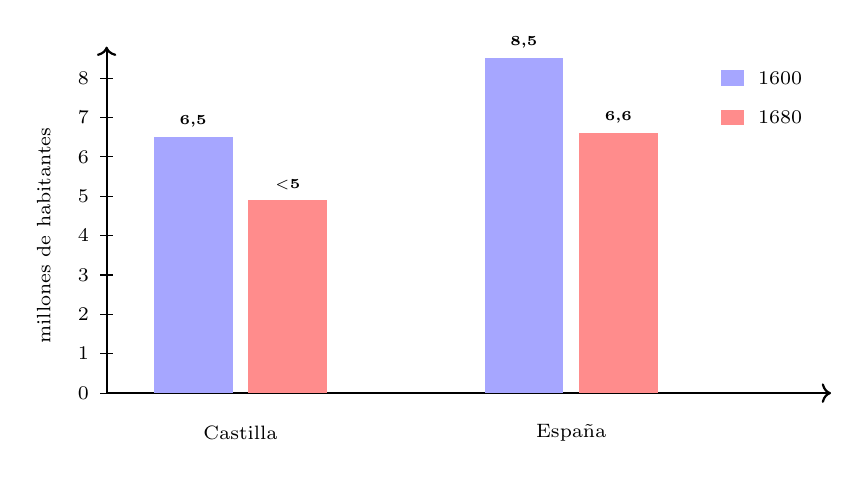
\begin{tikzpicture}

\draw[->, thick] (0,0) -- (0,4.4); \draw[->, thick] (0,0) -- (9.2,0);
\node[font=\scriptsize, rotate=90] at (-0.8,2.0) {millones de habitantes};
\foreach \y/\l in {0/0,0.5/1,1.0/2,1.5/3,2.0/4,2.5/5,3.0/6,3.5/7,4.0/8} { \draw (-0.08,\y) -- (0.08,\y); \node[font=\scriptsize, anchor=east] at (-0.1,\y) {\l}; }
\fill[blue!35] (0.6,0) rectangle (1.6,3.25); \fill[red!45] (1.8,0) rectangle (2.8,2.45);
\fill[blue!35] (4.8,0) rectangle (5.8,4.25); \fill[red!45] (6.0,0) rectangle (7.0,3.3);
\node[font=\tiny\bfseries] at (1.1,3.45) {6,5}; \node[font=\tiny\bfseries] at (2.3,2.65) {$<$5};
\node[font=\tiny\bfseries] at (5.3,4.45) {8,5}; \node[font=\tiny\bfseries] at (6.5,3.5) {6,6};
\node[font=\scriptsize] at (1.7,-0.5) {Castilla}; \node[font=\scriptsize] at (5.9,-0.5) {España};
\fill[blue!35] (7.8,3.9) rectangle (8.1,4.1); \node[font=\scriptsize, anchor=west] at (8.15,4.0) {1600};
\fill[red!45] (7.8,3.4) rectangle (8.1,3.6); \node[font=\scriptsize, anchor=west] at (8.15,3.5) {1680};

\end{tikzpicture}
\end{document}
